\documentclass[12pt,titlepage]{article}
\usepackage[margin=1.25in]{geometry}
\usepackage{fancyhdr,tabularx,graphicx,tikz,amsmath}
\usetikzlibrary{svg.path,calc}
\tikzstyle{square} = [rectangle, draw, text centered, minimum height=2em, minimum width=5cm]
\tikzstyle{arrow} = [line width=0.5mm,->]

\pagestyle{fancy}
\setlength{\headheight}{14.49998pt} % compensate fancyhdr style
\fancyhead{}
\fancyfoot{}
\fancyfoot[L]{\thepage}
\fancyfoot[R]{\textit{Basic Programming Practicum - Jobsheet 2}}
\renewcommand{\footrulewidth}{0.4pt}% default is 0pt, overline for footer

\newcommand{\details}[2]{
#1 & #2  \\
}

\begin{document}
\begin{titlepage}
    \centering
    \vfill
    {\bfseries\LARGE
        Basic Programming Practicum\\
        \vskip0.25cm
        Jobsheet 2
    }
    \vfill
    
\includegraphics[width=6cm]{images/polinema-logo.png}
    \vfill
    {\textbf{Name}\\
        Dicha Zelianivan Arkana\\
        \vskip0.5cm
        \textbf{NIM}\\
        2241720002\\
        \vskip0.5cm
        \textbf{Class}\\
        1i\\
        \vskip0.5cm
        \textbf{Department}\\
        Information Technology\\
        \vskip0.5cm
        \textbf{Study Program}\\
        D-IV Informatics Engineering}
\end{titlepage}

\section{Practice}
\subsection{Experiment 1: Complete a Case Study On Sequence}
\textbf{Questions}
\begin{enumerate}
    \item {
        Mention sequentially what you do after college like experiment 1 question-1!

        \begin{itemize}
            \item Pack my belongings like laptop, charger, etc.
            \item Get out of the classroom
            \item Go to the elevator or walk down the stairs
            \item Walk to the boarding house
            \item After arriving, take of my shoes, change my shirt, take a shower if it's already late
        \end{itemize}
    }

    \item {
        Rewrite and complete the algorithm in Experiment 1 No. 2!

        \begin{itemize}
            \item From the start the frog jumps in the 0 direction
            \item Then jump again in the 0 direction
            \item Then the frog turns to the lilly pad in the 6 direction
            \item After turning, the frog jumps 3 times
            \item Then the frog turns to the lilly pad in the 4 direction
            \item After turning, the frog jumps twice
            \item After that, the frog turns to the lilly pad in the 2 direction
            \item Then the frog jumps twice
            \item After jumping twice, the frog turns to the 4 direction
            \item After that, the frog jumps twice again
            \item Finally, the frog turns to the lilly pad in the 1 direction and jumps once
        \end{itemize}
    }
    \pagebreak
    \item {
        Calculate mathematically the results of experiment 1 problem 3! What is the result?

        \begin{tabularx}{\textwidth}[t]{@{}>{\bfseries}l!{:}X}
        \details{Input}{Periphery of Mr Ahmad's land, which is 64m}
        \details{Output}{Land Area}
        \details{Other Data}{-}
        \details{Process}{
            \begin{itemize}
                \item Enter the circumference of the land
                \item Calculate the length of sides from Mr Ahmad's land. $$side = perimeter \div 4 \rightarrow 64 \div 4 = \textbf{16}$$
                \item Calculate area. $$side \times side \rightarrow 16 \times 16 = \textbf{256}$$
                \item Pak ahmad's land area as an output.
            \end{itemize}
        }
        \end{tabularx}
    }
    \item {
        If there is additional information as follows
        "Mr. Ahmad wants to plant a circular rose in the middle of his land. Pak Ahmad wants
        to maximize his land so that as much as possible there are only a few vacant lands.
        What is the area of Mr. Ahmad's land planted with Mawar flowers? "
        Rewrite the steps for making the correct algorithm!

        \begin{tabularx}{\textwidth}[t]{@{}>{\bfseries}l!{:}X}
        \details{Input}{Mr Ahmad's land area, which is $256m^2$}
        \details{Output}{Land Area planted with Mawar flowers in circular shape}
        \details{Other Data}{-}
        \details{Process}{
            \begin{itemize}
                \item Enter the area of the land
                \item Calculate the area of circular shape inside Mr Ahmad's land.
                    We can use $\frac{1}{2} \times 16 = 8$ as the circle's radius
                \item Calculate area.
                    $$\pi r^2 = 3.14 \times 8^2 = \textbf{201}$$
                \item Pak ahmad's flower area, which is $\textbf{201}m^2$
            \end{itemize}
        }
        \end{tabularx}
    }
    \pagebreak
    \item {
        After additional data about question 4, what is the area of Mr. Ahmad's land that is not planted with roses?

        \begin{tabularx}{\textwidth}[t]{@{}>{\bfseries}l!{:}X}
        \details{Input}{Mr Ahmad's land area, which is $256m^2$, and flower area, $201m^2$}
        \details{Output}{Land Area that is not planted with Mawar flowers}
        \details{Other Data}{-}
        \details{Process}{
            \begin{itemize}
                \item Enter the area of the land
                \item Calculate the leftover area.
                    $$land~area-flower~area=256-201=\textbf{55}m^2$$
                \item Pak ahmad's land area that is not planted with flower, which is $\textbf{55}m^2$
            \end{itemize}
        }
        \end{tabularx}
    }
\end{enumerate}

\subsection{Experiment 2: Complete a Case Study About Selection}
\textbf{Questions}
\begin{enumerate}
    \item {
        Rewrite and complete the algorithm in experiment 2! \textcolor{gray}{(see next page)}

        \begin{tabularx}{\textwidth}[t]{@{}>{\bfseries}l!{:}X}
        \details{Input}{River, River connectivity information (For example, A is adjacent to B and D)}
        \details{Output}{Path of the entire river}
        \details{Other Data}{-}
        \details{Process}{
            \begin{itemize}
                \item Beaver is in the middle of several river meetings. He can swim from the river B / D / E / F / G
                \item {
                    If starting from \textbf{B} then the track that can be traversed by choosing river A or C.
                    If it crosses river A, then:
                    \begin{itemize}
                        \item River A continues to river D
                        \item From D has the option to E / F / G river. If you choose F or G then it is possibility that one river must be crossed more than once.
                            Then the river E was chosen
                        \item From E, proceed to the connected and have same direction river, river H
                        \item From the river H continued to the river that is connected and have same direction,
                            there are \textbf{F-G-C}
                        \item So the path Beaver goes through is \textbf{B-C-G-F-H-E-D-A} (output)
                    \end{itemize}
                    If it crosses river C, then:
                    \begin{itemize}
                        \item River C continues to river G
                        \item There are three other path, which is B, D, and E, but those are not what we want because it will make the beaver go the same river twice later on.
                            So we choose to go to \textbf{F-H-E}
                        \item Then the only path left is \textbf{D-A}
                        \item So the path Beaver goes through is \textbf{A-D-E-H-F-G-C}
                    \end{itemize}
                }
                \item {
                    If it starts from D then the track that can be traversed by choosing river A.
                    \begin{itemize}
                        \item From river A, there are 2 choices, B and C. Let's choose the path from C, which makes the beaver go through \textbf{C-G}
                        \item Now, there are several choices (B / E / F). We can't choose B because we'll be going through the same river twice.
                            We'll choose F because choosing it will make the entire path simpler.
                        \item After choosing F, we'll go through \textbf{F-H-E}
                        \item The only river left is B, so choose that.
                        \item So the path Beaver goes through is \textbf{B-E-H-F-G-C-A}
                    \end{itemize}
                }
            \end{itemize}
        }
        \end{tabularx}
    }
    \item {
        \begin{tabularx}{\textwidth}[t]{@{}>{\bfseries}l!{:}X}
        \details{~~~~~~~~~~~~~~~~}{
            \begin{itemize}
                \item {
                    If it starts from E then the track that can be traversed by choosing river H.
                    \begin{itemize}
                        \item From river H, the only option is to go through F
                        \item There are several options that we can go from river F (D / B / G),
                            choose river G just because it's the next letter after F.
                        \item After choosing G, we can go through \textbf{G-C}
                        \item Now, we have two options, A and B. Choose B.
                        \item After we go to B, there is only one path left, which is \textbf{D-A}
                        \item So the path Beaver goes through is \textbf{A-D-B-C-G-F-H-E}
                    \end{itemize}
                }
                \item {
                    If it starts from F then the track that can be traversed by choosing river H.
                    \begin{itemize}
                        \item From river H, we can go through \textbf{H-E}
                        \item There are several options that we can choose (D / B / G).
                            Choose D just because it's the letter that comes before E
                        \item After choosing D, we can then go to A
                        \item Here, we can choose between B and C.
                            We can choose B just because it's the letter that comes after A
                        \item There is only one path left, which is \textbf{G-C}
                        \item So the path Beaver goes through is \textbf{C-G-B-A-D-E-H-F}
                    \end{itemize}
                }
                \item {
                    If it starts from G then the track that can be traversed by choosing river C.
                    \begin{itemize}
                        \item After arriving at river C, we can choose between A and B. Choose \textbf{A-D}
                        \item Now, We have several options (B / E / F), choose F because it's a straight path.
                        \item We can then go through \textbf{F-H-E}
                        \item There's only one path left, which is B
                        \item So the path Beaver goes through is \textbf{B-E-H-F-D-A-C-G}
                    \end{itemize}
                }
            \end{itemize}
        }
        \end{tabularx}
    }
    \pagebreak
    \setcounter{enumi}{1}
    \item {
        Write the algorithm of the regulation SP1, SP2, and SP3 at JTI Polinema as you know!
        
        This answer assumes that the student have 20 hours of alpha

        \begin{tabularx}{\textwidth}[t]{@{}>{\bfseries}l!{:}X}
            \details{Input}{Student's alpha total, which is 20 hours}
            \details{Output}{What type of SP the student will get}
            \details{Other Data}{-}
            \details{Process}{
                \begin{itemize}
                    \item Check the student's alpha total
                    \item If it's $>=$ 18 hours, then the student will get SP1
                    \item If it's $>=$ 36 hours, then the student will get SP2
                    \item If it's $>=$ 47 hours, then the student will get SP3
                    \item Otherwise, the student won't get anything
                    \item Since the student has 20 hours of alpha, the student will get SP1
                \end{itemize}
            }
        \end{tabularx}
       
    }
\end{enumerate}

\subsection{Experiment 3: Complete a Case Study About Repetition}
\textbf{Questions}
\begin{enumerate}
    \item {
        Mention the position that was detected wrongly in experiment 3 questions 2!\\
        The beaver that sits at the wrong place is the beaver at \texttt{[3,4]} because that beaver should be sitting at \texttt{[4,3]}
    }
    \item {
        Mention 5 activities that use the concept of repetition / looping that you have encountered!

        \begin{enumerate}
            \item Doing the laundry
            \item Rinsing rice
            \item Washing the dishes
            \item Coding
            \item Designing
        \end{enumerate}
    }
\end{enumerate}

\pagebreak

\section{Assignment}

\begin{enumerate}
    \item {
        \begin{figure}[h]
            \centering
            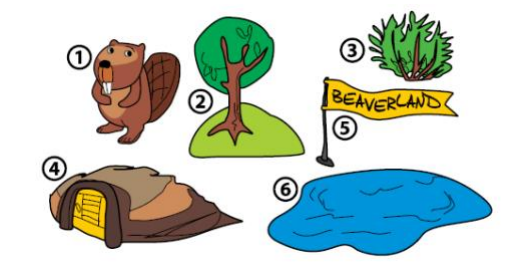
\includegraphics[width=8cm]{images/figure6.png}
            \caption{The painting that Lina wanted}
            \label{fig:stamps}
        \end{figure}
        \begin{figure}[h]
            \centering
            
\includegraphics[width=8cm]{images/figure7.png}
            \caption{The painting that Lina wanted}
            \label{fig:painting}
        \end{figure}
        Create an algorithm to get a painting like the one above (shown by figure 2)!

        \begin{tabularx}{\textwidth}[t]{@{}>{\bfseries}l!{:}X}
        \details{Input}{Stamps as shown on figure 1}
        \details{Output}{Painting as shown on figure 2}
        \details{Other Data}{-}
        \details{Process}{
            \begin{itemize}
                \item Use \textit{the pond} (6) as the first layer because it has the most cut-off part
                \item The next layer would be \textit{the island with a tree} (2)
                \item The third layer is \textit{the beaverland flag} (5)
                \item The next layer is going to be \textit{the beaver house} (4)
                \item Add \textit{the bush} (3) as the fourth layer
                \item Finally, add \textit{the beaver} (1) as the top-most layer
            \end{itemize}
        }
        \end{tabularx}
    }
    \pagebreak
    \item {
        \begin{figure}[h]
            \centering
            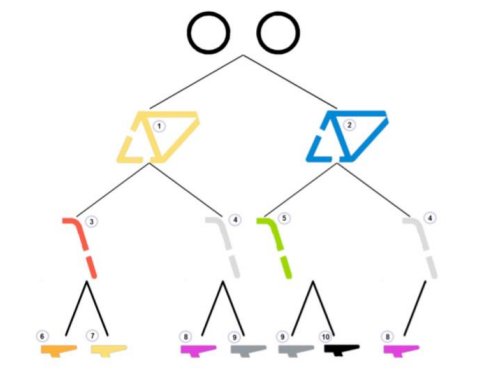
\includegraphics[width=8cm]{images/figure8.png}
            \caption{Bicycle color rule}
            \label{fig:bike-parts}
        \end{figure}
        \begin{figure}[h]
            \centering
            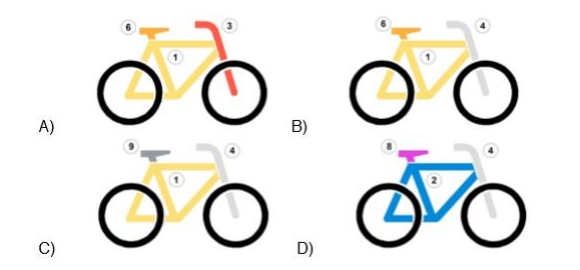
\includegraphics[width=8cm]{images/figure9.png}
            \caption{Bicycle results}
            \label{fig:bike-final}
        \end{figure}
        In accordance with the above rules, which of the following bikes (shown by figure 4) is unsuitable?

        \begin{tabularx}{\textwidth}[t]{@{}>{\bfseries}l!{:}X}
        \details{Input}{Bicycle color rule as (shown on figure 3), Bicycle result to choose from (shown on figure 4)}
        \details{Output}{Unsuitable combination}
        \details{Other Data}{-}
        \details{Process}{
            \begin{itemize}
                \item Check the first part, every bicycle can have a pair of tire. Every bicycle have a pair of tire.
                \item Next step is to check the bicycle body, which is yellow and blue. Every bicycle have a correct body part.
                \item After choosing the body, choose the handle. Every bicycle has the correct handle according to the rule.
                \item Some bicycle with specific handle can only choose specific saddle. If we check the bicycles, we can see that the bicycle \textbf{(B)} uses an incorrect saddle.
                    It can only choose between pink or grey if it has a white handle but it uses a yellow saddle.
            \end{itemize}
        }
        \end{tabularx}
    }
    \pagebreak
    \item {
        Do interviews with students in the same class (choose 5-10 students) as you! Record
        information about nickname, blood group, date of birth, month of birth, hometown,
        and hobby. Present the information in a network:
        \vspace{0.5cm}

        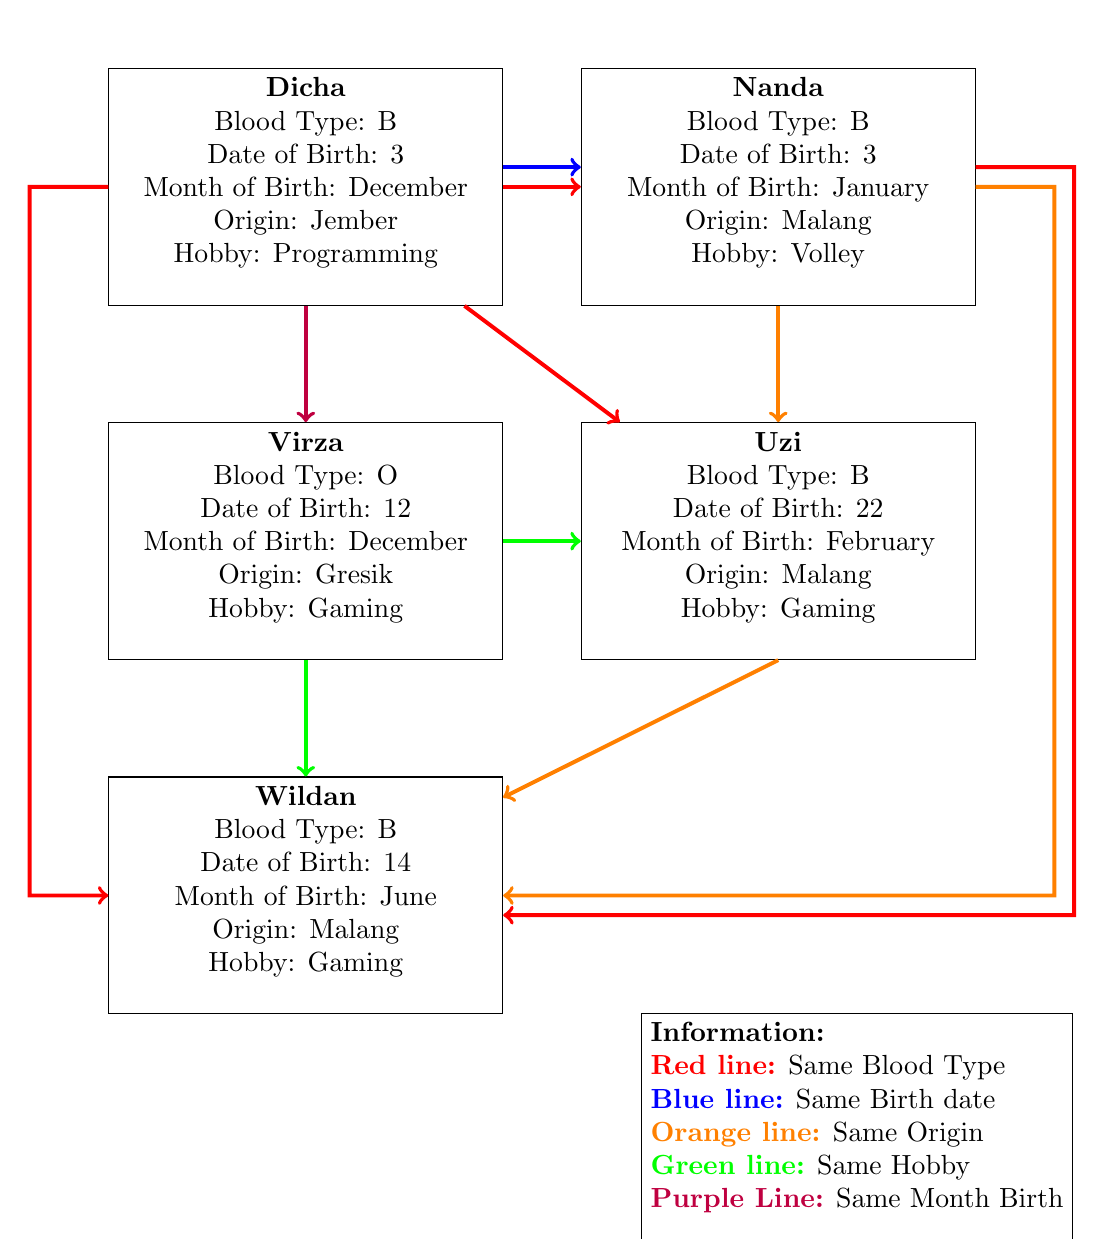
\begin{tikzpicture}[node distance=2cm]
            \node (p1) [square, align=center] {
                \textbf{Dicha}\\
                Blood Type: B\\
                Date of Birth: 3\\
                Month of Birth: December\\
                Origin: Jember\\
                Hobby: Programming\\
            };
            \node (p2) [square, align=center, right of = p1, xshift=4cm] {
                \textbf{Nanda}\\
                Blood Type: B\\
                Date of Birth: 3\\
                Month of Birth: January\\
                Origin: Malang\\
                Hobby: Volley\\
            };
            \node (p3) [square, align=center, below of = p1, yshift=-2.5cm] {
                \textbf{Virza}\\
                Blood Type: O\\
                Date of Birth: 12\\
                Month of Birth: December\\
                Origin: Gresik\\
                Hobby: Gaming\\
            };
            \node (p4) [square, align=center, below of = p2, yshift=-2.5cm] {
                \textbf{Uzi}\\
                Blood Type: B\\
                Date of Birth: 22\\
                Month of Birth: February\\
                Origin: Malang\\
                Hobby: Gaming\\
            };
            \node (p5) [square, align=center, below of = p3, yshift=-2.5cm] {
                \textbf{Wildan}\\
                Blood Type: B\\
                Date of Birth: 14\\
                Month of Birth: June\\
                Origin: Malang\\
                Hobby: Gaming\\
            };
            \node (info) [square, align=left, below of = p4, yshift=-5.5cm, xshift=1cm] {
                \textbf{Information:}\\
                \textbf{\textcolor{red}{Red line:}} Same Blood Type\\
                \textbf{\textcolor{blue}{Blue line:}} Same Birth date\\
                \textbf{\textcolor{orange}{Orange line:}} Same Origin\\
                \textbf{\textcolor{green}{Green line:}} Same Hobby\\
                \textbf{\textcolor{purple}{Purple Line:}} Same Month Birth\\
            };
            \draw [arrow, red] (p1) -- (p2);
            \draw [arrow, red] (p1) -- (p4);
            \draw [arrow, red] (p1.west) -- ($(p1.west)-(1cm,0)$) -- ($(p1.west)-(1cm,9cm)$) -- (p5.west);
            \draw [arrow, blue] ($(p1.east)+(0,0.25cm)$) -- ($(p2.west)+(0,0.25cm)$);
            \draw [arrow, purple] (p1) -- (p3);
            \draw [arrow, orange] (p2.east) -- ($(p2.east)+(1cm,0)$) -- ($(p4.east)+(1cm,-4.5cm)$) -- (p5);
            \draw [arrow, red] ($(p2.east)+(0,0.25cm)$) -- ($(p2.east)+(1.25cm,0.25cm)$) -- ($(p4.east)+(1.25cm,-4.75cm)$) -- ($(p5.east)+(0,-0.25cm)$);
            \draw [arrow, orange] (p2) -- (p4);
            \draw [arrow, green] (p3) -- (p4);
            \draw [arrow, green] (p3) -- (p5);
            \draw [arrow, orange] (p4.south) -- (p5);
        \end{tikzpicture}
        \pagebreak\\
        {
            Then answer the following questions
            \begin{enumerate}
                \item {
                    Who has the same blood type as you?
                    \begin{itemize}
                        \item Nanda
                        \item Uzi
                        \item Wildan
                    \end{itemize}
                }
                \item {
                    Who were born in the same month as you?
                    \begin{itemize}
                        \item Virza
                    \end{itemize}
                }
                \item {
                    Who was born on the same date as you?
                    \begin{itemize}
                        \item Nanda
                    \end{itemize}
                }
                \item {
                    Who are from the same area as you?
                    \begin{itemize}
                        \item -
                    \end{itemize}
                }
                \item {
                    Who has the same hobby as you?
                    \begin{itemize}
                        \item -
                    \end{itemize}
                }
            \end{enumerate}
        }
    }
    \item {
        A laundry service "Smile Laundry" has a fee rule like this one
        \begin{itemize}
            \item The fare for every 1 kg of clothing is Rp. 4,500
            \item If the customer washes clothes more than 10 kg, the customer will get a 5\% discount
        \end{itemize}
        Today, Laundry only has 4 customers, namely Ani, Budi, Bina, and Cita.
        Ani brought 4kg of clothes, Budi brought 15kg of clothes, Bina brought 2kg, and finally Cita brought 11kg.
        What did Smile Laundry think that day? Create the Algorithm!

        \begin{tabularx}{\textwidth}[t]{@{}>{\bfseries}l!{:}X}
            \details{Input}{Laundry price/kg, Ani clothes (4kg), Budi clothes (15kg), Bina clothes (2kg), and Cita clothes (11kg)}
            \details{Output}{The total price}
            \details{Other Data}{5\% discount every $>10kg$}
            \details{Process}{
                \begin{itemize}
                    \item {
                        Calculate each prices using multiplication. If amount $>10kg$ then apply the discount
                        \begin{align}
                            Ani &= 4 \times 4500 &=& \textbf{Rp.18.000,-}\\
                            Budi &= 15 \times 4500 - (5\%) = 67500 - 3375 &=& \textbf{Rp.64.125,-}\\
                            Bina &= 2 \times 4500 &=& \textbf{Rp.9.000,-}\\
                            Cita &= 11 \times 45000 - (5\%) = 49500 - 2475 &=& \textbf{Rp.47.025,-}
                        \end{align}
                    }
                    \item {
                        Sum the prices
                        \begin{align}
                            18000+64125+9000+47025 = \textbf{Rp.138.150,-}
                        \end{align}
                        So the total price is $\textbf{Rp.138.150,-}$
                    }
                \end{itemize}
            }
        \end{tabularx}
    }
\end{enumerate}

\end{document}

